\appendix
\appendixpage
\addappheadtotoc
\setcounter{equation}{0}

\section{Tables of Results}


\begin{table}[width=15cm]
 \begin{center}
\resizebox{16cm}{!} {
\begin{tabular}{|c|c|c|c|c|r|r|r|} \hline
\multicolumn{2}{|c|}{} & $\langle-t\rangle$ & $\langle
x_{\text{B}}\rangle$ & $\langle Q^2 \rangle $ & 
\multicolumn{1}{c|}{\multirow{2}{*}{$A_{\text{LU,I}}^{\sin \phi} \pm \delta_{stat.} \pm \delta_{syst.}$}} & 
\multicolumn{1}{c|}{\multirow{2}{*}{$A_{\text{LU,DVCS}}^{\sin \phi} \pm \delta_{stat.} \pm \delta_{syst.}$}} & 
\multicolumn{1}{c|}{\multirow{2}{*}{$A_{\text{LU,I}}^{\sin (2\phi)} \pm \delta_{stat.} \pm \delta_{syst.}$}} \\ 
\multicolumn{2}{|c|}{} &  $[\text{GeV}^2]$ & & $[\text{GeV}^2]$ & &  &  \\
\hline \hline
\multicolumn{2}{|c|}{overall} &  0.117 & 0.097 &  2.52 &  -0.222  $\pm$  0.023  $\pm$   0.022 &
 0.005  $\pm$  0.023  $\pm$  0.003 & 0.005  $\pm$  0.023  $\pm$   0.003 \\
\hline
\multirow{6}{*}{\rotatebox{90}{\mbox{$t [\text{GeV}^2]$}}} & 0.00-0.03 &  0.018 & 0.068 &  1.72 &  -0.217  $\pm$  0.051  $\pm$   0.010 &
 0.031  $\pm$  0.051   $\pm$  0.003 & -0.032  $\pm$  0.051  $\pm$   0.003\\
& 0.03-0.06 &  0.043 & 0.088 &  2.26&  -0.222 $\pm$   0.052   $\pm$  0.014 &
 -0.024 $\pm$   0.052  $\pm$   0.006 & 0.062  $\pm$  0.052  $\pm$   0.002\\
& 0.06-0.10 &  0.078 & 0.099 &  2.51 & -0.163 $\pm$   0.057   $\pm$  0.012 &
 -0.010  $\pm$  0.056  $\pm$   0.005 & 0.039  $\pm$  0.056   $\pm$  0.006 \\
& 0.10-0.20 &  0.142 & 0.110 &  2.79 &  -0.246 $\pm$   0.049  $\pm$   0.011 &
0.007  $\pm$  0.049  $\pm$   0.003 & 0.007  $\pm$  0.049  $\pm$  0.008\\
& 0.20-0.35 &  0.260 & 0.121 &  3.27 &  -0.297 $\pm$   0.066  $\pm$   0.006 &
0.086  $\pm$  0.066  $\pm$   0.003 & -0.035 $\pm$   0.066   $\pm$  0.008\\
& 0.35-0.70 &  0.460 & 0.125 &  3.82 &  -0.189  $\pm$  0.095  $\pm$   0.015 & 
-0.111  $\pm$  0.095   $\pm$  0.024 & -0.056 $\pm$   0.096  $\pm$   0.029\\
\hline
\multirow{6}{*}{\rotatebox{90}{\mbox{$x_{\text{B}}$}}} & 0.03-0.06 &  0.095 & 0.049 &  1.34 &  -0.237  $\pm$  0.050  $\pm$   0.076 &
0.002 $\pm$   0.050  $\pm$   0.005 & -0.064  $\pm$  0.051  $\pm$   0.010\\
& 0.06-0.08 &  0.091 & 0.069 &  1.80 &  -0.235  $\pm$  0.050  $\pm$   0.047 &
0.010 $\pm$  0.050  $\pm$   0.004 & 0.024 $\pm$   0.049  $\pm$   0.012\\
& 0.08-0.10 &  0.104 & 0.089 &  2.30 &  -0.263 $\pm$  0.057  $\pm$   0.033 &
0.069 $\pm$   0.056  $\pm$   0.004 & 0.028  $\pm$  0.056  $\pm$   0.007\\
& 0.10-0.13 &  0.121 &  0.113 &  2.93 &  -0.223  $\pm$  0.059   $\pm$  0.030 & 
-0.015  $\pm$  0.058  $\pm$   0.007 & -0.012  $\pm$  0.059  $\pm$   0.010\\
& 0.13-0.20 &  0.159 & 0.157 &  4.06&  -0.216  $\pm$  0.063  $\pm$   0.013 &
0.014  $\pm$  0.063  $\pm$   0.006 & 0.046  $\pm$  0.061  $\pm$   0.010 \\
& 0.20-0.35 &  0.231 & 0.244 &  6.14 &  -0.113 $\pm$ 0.110  $\pm$   0.021 &
-0.111  $\pm$  0.110 $\pm$    0.017 & 0.046  $\pm$  0.102  $\pm$  0.015\\
\hline
\multirow{6}{*}{\rotatebox{90}{\mbox{$Q^2 [\text{GeV}^2]$}}} & 1.00-1.40 &  0.076 & 0.054  & 1.20 &  -0.193  $\pm$  0.051  $\pm$   0.061 &
-0.001 $\pm$   0.051  $\pm$   0.002 & -0.020  $\pm$  0.051   $\pm$  0.010 \\
& 1.40-1.80 &  0.089 & 0.069 &  1.59 &  -0.311 $\pm$  0.055  $\pm$   0.062 &
0.047  $\pm$  0.055  $\pm$   0.011 & -0.021 $\pm$   0.054  $\pm$   0.005\\
& 1.80-2.40 &  0.104 & 0.085 &  2.08 &  -0.224 $\pm$   0.051  $\pm$   0.042 &
0.014 $\pm$   0.051  $\pm$   0.005 & 0.015  $\pm$  0.053  $\pm$   0.008\\
& 2.40-3.20 &  0.126 & 0.105  & 2.77 &  -0.219 $\pm$   0.054  $\pm$   0.044 &
0.010  $\pm$  0.054 $\pm$    0.007 & 0.028   $\pm$ 0.049  $\pm$   0.006\\
& 3.20-4.50 &  0.151 & 0.134 &  3.76 &  -0.180 $\pm$   0.063  $\pm$   0.031 &
-0.025  $\pm$  0.062 $\pm$    0.006 & -0.016 $\pm$   0.062  $\pm$   0.008\\
& 4.50-10.0 &  0.218 & 0.200 &  5.82 &  -0.200  $\pm$  0.074 $\pm$    0.004 &
-0.036  $\pm$  0.074  $\pm$   0.007 & 0.069 $\pm$  0.071$ \pm$  0.013\\
\hline
  \end{tabular}
}
 \end{center}
\caption{Results of the $A_{\textrm{LU,I}}^{\sin(n\phi)}$ and $A_{\textrm{LU,DVCS}}^{\sin \phi}$ asymmetry amplitudes with statistical and systematic uncertainties and average kinematics from unpolarised hydrogen target data taken during 2006-2007 at H{\sc ermes} for each $t$, $x_{\textrm{B}}$ and $Q^{2}$ bin. An additional 3.4\,\% scale uncertainty is present in the amplitudes due to the uncertainty of the beam polarisation measurement.}
\end{table}

\begin{table}[width=15cm]
 \begin{center}
\resizebox{16cm}{!} {
\begin{tabular}{|c|c|c|c|c|r|r|r|r|} \hline
\multicolumn{2}{|c|}{} & $\langle t\rangle$ & $\langle
x_{\text{B}}\rangle$ & $\langle Q^2 \rangle $ & 
\multicolumn{1}{c|}{\multirow{2}{*}{$A_{\text{C}}^{\cos (0\phi)}\pm \delta_{stat.} \pm \delta_{syst.}$ }} & 
\multicolumn{1}{c|}{\multirow{2}{*}{$A_{\text{C}}^{\cos \phi } \pm \delta_{stat.} \pm \delta_{syst.}$}} & 
\multicolumn{1}{c|}{\multirow{2}{*}{$A_{\text{C}}^{\cos (2\phi) } \pm \delta_{stat.} \pm \delta_{syst.}$ }} &
\multicolumn{1}{c|}{\multirow{2}{*}{$A_{\text{C}}^{\cos (3\phi) } \pm \delta_{stat.} \pm \delta_{syst.}$}} \\ 
\multicolumn{2}{|c|}{} &  $[\text{GeV}^2]$ & & $[\text{GeV}^2]$ & &  & &  \\
\hline
\hline
\multicolumn{2}{|c|}{overall} &  0.117 & 0.097 &  2.52 &  -0.024 $\pm$  0.004 $\pm$  0.011 & 
0.032  $\pm$  0.006 $\pm$   0.002 &  -0.004  $\pm$  0.005  $\pm$   0.014 &  0.001  $\pm$   0.005   $\pm$   0.004 \\
\hline
\multirow{6}{*}{\rotatebox{90}{\mbox{$t [\text{GeV}^2]$}}} & 0.00-0.03 &  0.018 & 0.068 &  1.72 &  -0.014  $\pm$  0.009 $\pm$ 0.007 & 
0.006  $\pm$  0.012  $\pm$   0.003 &  -0.038  $\pm$  0.012 $\pm$  0.001 &  -0.022   $\pm$  0.012   $\pm$   0.004\\
& 0.03-0.06 &  0.043 & 0.088 &  2.26& -0.008  $\pm$  0.009  $\pm$   0.006 &
0.016 $\pm$  0.012  $\pm$   0.014 &  -0.004  $\pm$  0.012  $\pm$  0.007 &  0.003   $\pm$  0.012   $\pm$   0.005\\
& 0.06-0.10 &  0.078 & 0.099 &  2.51 & -0.025  $\pm$  0.009  $\pm$  0.007 & 
0.030 $\pm$  0.013  $\pm$   0.013 & 0.011  $\pm$  0.012 $\pm$   0.013 &  -0.028   $\pm$  0.012  $\pm$    0.004\\
& 0.10-0.20 &  0.142 & 0.110 &  2.79 &  -0.019  $\pm$  0.008   $\pm$  0.010 & 
0.036 $\pm$  0.012  $\pm$   0.014 &  0.007  $\pm$  0.011  $\pm$  0.025 & 0.019   $\pm$  0.011    $\pm$  0.001\\
& 0.20-0.35 &  0.260 & 0.121 &  3.27 &  -0.042 $\pm$   0.011  $\pm$  0.004 &
0.078 $\pm$  0.016  $\pm$ 0.029 & -0.016 $\pm$   0.015  $\pm$  0.040 & 0.023  $\pm$   0.015   $\pm$   0.001\\
& 0.35-0.70 &  0.460 & 0.125 &  3.82 &  -0.083  $\pm$  0.016  $\pm$   0.005 & 
0.069 $\pm$  0.025  $\pm$   0.061 & 0.052 $\pm$   0.022  $\pm$  0.040 & 0.030   $\pm$  0.021   $\pm$ 0.017\\
\hline
\multirow{6}{*}{\rotatebox{90}{\mbox{$x_{\text{B}}$}}} & 0.03-0.06 &  0.095 & 0.049 &  1.34 &  -0.038  $\pm$  0.009  $\pm$   0.013 & 
 0.007  $\pm$  0.013  $\pm$   0.013 & -0.026 $\pm$  0.012 $\pm$   0.013 &  -0.015   $\pm$  0.011  $\pm$    0.003\\
& 0.06-0.08 &  0.091 & 0.069 &  1.80&   -0.046  $\pm$  0.008  $\pm$   0.012 &
0.025  $\pm$  0.012  $\pm$   0.013 & -0.001  $\pm$ 0.011  $\pm$   0.009 & -0.003   $\pm$  0.011   $\pm$   0.005\\
& 0.08-0.10 &  0.104 & 0.089 &  2.30 &  -0.004  $\pm$  0.010  $\pm$   0.016 & 
0.033  $\pm$  0.014  $\pm$   0.019 & -0.013 $\pm$  0.013 $\pm$    0.017 & -0.013   $\pm$  0.013    $\pm$  0.002\\
& 0.10-0.13 &  0.121 &  0.113 &  2.93 &  -0.025  $\pm$  0.010  $\pm$   0.015 & 
0.035  $\pm$  0.014 $\pm$   0.002 & -0.015 $\pm$  0.013  $\pm$   0.006 & 0.001   $\pm$  0.013  $\pm$    0.009\\
& 0.13-0.20 &  0.159 & 0.157 &  4.06&   -0.012   $\pm$ 0.011  $\pm$   0.007 & 
0.029  $\pm$  0.015 $\pm$    0.031 & -0.003  $\pm$  0.014  $\pm$   0.001 & 0.016   $\pm$  0.014   $\pm$  0.005\\
& 0.20-0.35 &  0.231 & 0.244 &  6.14 &  -0.009 $\pm$  0.018   $\pm$  0.026 & 
0.060  $\pm$  0.026   $\pm$    0.018 & 0.069  $\pm$  0.024  $\pm$ 0.027 & 0.043  $\pm$   0.024  $\pm$   0.009\\
\hline
\multirow{6}{*}{\rotatebox{90}{\mbox{$Q^2 [\text{GeV}^2]$}}} & 1.00-1.40 &  0.076 & 0.054  & 1.20 &  -0.046  $\pm$  0.008  $\pm$   0.023 & 
0.021  $\pm$  0.012  $\pm$   0.028 &  -0.020 $\pm$  0.011  $\pm$  0.012 & -0.014  $\pm$  0.011   $\pm$   0.004\\
& 1.40-1.80 &  0.089 & 0.069 &  1.59 &  -0.018  $\pm$  0.009  $\pm$   0.021 & 
0.032  $\pm$  0.013  $\pm$   0.020 & -0.011  $\pm$  0.012  $\pm$  0.012 & 0.001  $\pm$  0.012   $\pm$  0.002\\
& 1.80-2.40 &  0.104 & 0.085 &  2.08 &  -0.039  $\pm$  0.009  $\pm$   0.022 &
0.016  $\pm$  0.012  $\pm$   0.017 & -0.008 $\pm$   0.012  $\pm$  0.013 & 0.018  $\pm$   0.012  $\pm$  0.004\\
& 2.40-3.20 &  0.126 & 0.105  & 2.77 &  -0.016 $\pm$   0.010  $\pm$   0.019 &  
0.068  $\pm$  0.014  $\pm$   0.020 & 0.006  $\pm$  0.013  $\pm$  0.013 & -0.022  $\pm$  0.013  $\pm$  0.009\\
& 3.20-4.50 &  0.151 & 0.134 &  3.76 &  0.002  $\pm$  0.011   $\pm$  0.014 & 
0.010 $\pm$   0.015  $\pm$   0.002 & -0.008  $\pm$  0.014 $\pm$ 0.015 & 0.014   $\pm$  0.014  $\pm$  0.002\\
& 4.50-10.0 &  0.218 & 0.200 &  5.82 &  -0.003  $\pm$  0.013  $\pm$   0.014 & 
0.037  $\pm$  0.018  $\pm$  0.038 & 0.042 $\pm$   0.017  $\pm$  0.003 & 0.010   $\pm$  0.017   $\pm$   0.005\\
\hline
  \end{tabular}
}
 \end{center}
\caption{Results of the $A_{\textrm{C}}^{\cos(n\phi)}$ asymmetry amplitudes with statistical and systematic uncertainties and average kinematics from unpolarised hydrogen target data taken during 2006-2007 at H{\sc ermes} for each $t$, $x_{\textrm{B}}$ and $Q^{2}$ bin.}
\end{table}


\begin{table}[width=15cm]
 \begin{center}
\resizebox{16cm}{!} {
\begin{tabular}{|c|c|c|c|c|r|r|r|} \hline
\multicolumn{2}{|c|}{} & $\langle t\rangle$ & $\langle
x_{\text{B}}\rangle$ & $\langle Q^2 \rangle $ & 
\multicolumn{1}{c|}{\multirow{2}{*}{$A_{\text{LU,I}}^{\sin \phi} \pm \delta_{stat.} \pm \delta_{syst.}$}} & 
\multicolumn{1}{c|}{\multirow{2}{*}{$A_{\text{LU,DVCS}}^{\sin \phi} \pm \delta_{stat.} \pm \delta_{syst.}$ }} & 
\multicolumn{1}{c|}{\multirow{2}{*}{$A_{\text{LU,I}}^{\sin (2\phi)} \pm \delta_{stat.} \pm \delta_{syst.}$}} \\ 
\multicolumn{2}{|c|}{} &  $[\text{GeV}^2]$ & & $[\text{GeV}^2]$ & & &  \\
\hline \hline
\multicolumn{2}{|c|}{overall} &  0.118 & 0.097 &  2.51 &  -0.229  $\pm$  0.018  $\pm$   0.024 &
 0.017  $\pm$  0.018  $\pm$  0.001 & -0.010  $\pm$  0.018  $\pm$   0.001 \\
\hline
\multirow{6}{*}{\rotatebox{90}{\mbox{$t [\text{GeV}^2]$}}} & 0.00-0.03 &  0.019 & 0.069 &  1.72 &  -0.225  $\pm$  0.039 $\pm$   0.010 &
 0.048  $\pm$  0.039   $\pm$  0.003 & 0.003  $\pm$  0.039  $\pm$   0.003\\
& 0.03-0.06 &  0.044 & 0.088 &  2.25 &  -0.242 $\pm$   0.039   $\pm$  0.014 &
 0.019 $\pm$   0.039  $\pm$   0.005 & 0.026  $\pm$  0.038  $\pm$   0.001\\
& 0.06-0.10 &  0.079 & 0.099 &  2.49 & -0.177 $\pm$   0.043   $\pm$  0.012 &
 -0.023  $\pm$  0.043  $\pm$   0.004 & -0.002  $\pm$  0.043   $\pm$  0.005 \\
& 0.10-0.20 &  0.143 & 0.109 &  2.76 &  -0.253 $\pm$   0.037  $\pm$   0.010 &
0.010  $\pm$  0.037  $\pm$   0.002 & -0.008  $\pm$  0.037  $\pm$  0.006\\
& 0.20-0.35 &  0.261 & 0.119 &  3.23 &  -0.287 $\pm$   0.050  $\pm$   0.006 &
0.105  $\pm$  0.051  $\pm$   0.002 & -0.047 $\pm$   0.051   $\pm$  0.005\\
& 0.35-0.70 &  0.463 & 0.122 &  3.73 &  -0.173  $\pm$  0.072  $\pm$   0.016 & 
-0.107  $\pm$  0.073   $\pm$  0.023 & -0.111 $\pm$   0.074  $\pm$   0.028\\
\hline
\multirow{6}{*}{\rotatebox{90}{\mbox{$x_{\text{B}}$}}} & 0.03-0.06 &  0.099 & 0.049 & 1.34 & -0.249  $\pm$  0.038  $\pm$   0.079 &
0.035 $\pm$   0.038  $\pm$   0.004 & -0.044  $\pm$  0.039  $\pm$  0.011 \\ 
& 0.06-0.08 &  0.093 & 0.070 &  1.79 &  -0.228 $\pm$  0.037  $\pm$   0.049 &
0.013  $\pm$  0.038  $\pm$   0.002 & 0.023 $\pm$   0.037  $\pm$   0.012\\
& 0.08-0.10 &  0.106 & 0.089 &  2.30 &  -0.250 $\pm$   0.043  $\pm$   0.033 &
0.047 $\pm$   0.043  $\pm$   0.004 & 0.032  $\pm$  0.043  $\pm$   0.007\\
& 0.10-0.13 &  0.122 &  0.114 &  2.94 &  -0.237 $\pm$   0.045  $\pm$   0.030 &
-0.003  $\pm$  0.045 $\pm$    0.006 & -0.027 $\pm$ 0.045  $\pm$   0.010\\
& 0.13-0.20 &  0.160 & 0.157 &  4.06 &  -0.224 $\pm$   0.048  $\pm$   0.013 &
0.033  $\pm$  0.048 $\pm$    0.006 & -0.050 $\pm$   0.047  $\pm$   0.006\\
& 0.20-0.35 &  0.233 & 0.244 &  6.13 &  -0.077  $\pm$  0.085 $\pm$    0.022 &
-0.141  $\pm$  0.085  $\pm$   0.012 & -0.023 $\pm$  0.080 $ \pm$  0.007\\
\hline
\multirow{6}{*}{\rotatebox{90}{\mbox{$Q^2 [\text{GeV}^2]$}}} & 1.00-1.40 &  0.078 & 0.055  & 1.20  &  -0.218  $\pm$  0.038  $\pm$   0.063 &
0.029 $\pm$   0.038  $\pm$   0.002 & -0.023  $\pm$  0.038  $\pm$   0.012\\
& 1.40-1.80 &  0.092 & 0.069 &  1.59  &  -0.257  $\pm$  0.042  $\pm$   0.064 &
0.040 $\pm$  0.042  $\pm$   0.006 & 0.011 $\pm$   0.042  $\pm$   0.004\\
& 1.80-2.40 &  0.106 & 0.085 &  2.08  &  -0.233 $\pm$  0.041  $\pm$   0.042 &
0.016 $\pm$   0.041  $\pm$   0.004 & -0.010  $\pm$  0.040  $\pm$   0.007\\
& 2.40-3.20 &  0.127 & 0.105  & 2.77  &  -0.302  $\pm$  0.044   $\pm$  0.044 & 
0.087  $\pm$  0.044  $\pm$   0.006 & 0.031  $\pm$  0.044  $\pm$   0.005\\
& 3.20-4.50 &  0.152 & 0.134 &  3.77  &  -0.160  $\pm$  0.048  $\pm$   0.032 &
-0.057  $\pm$  0.048  $\pm$   0.005 & -0.061  $\pm$  0.048  $\pm$   0.004 \\
& 4.50-10.0 &  0.220 & 0.199 &  5.79  &  -0.169 $\pm$ 0.057  $\pm$   0.008 &
-0.065  $\pm$  0.057 $\pm$ 0.005 & -0.017  $\pm$  0.056  $\pm$  0.013\\
\hline
  \end{tabular}
}
 \end{center}
\caption{Results of the $A_{\textrm{LU,I}}^{\sin(n\phi)}$ and $A_{\textrm{LU,DVCS}}^{\sin \phi}$ asymmetry amplitudes with statistical and systematic uncertainties and average kinematics from unpolarised hydrogen target data taken during 1996-2007 at H{\sc ermes} for each $t$, $x_{\textrm{B}}$ and $Q^{2}$ bin.
An additional 3.2\,\% scale uncertainty is present in the amplitudes due to the uncertainty of the beam polarisation measurement.
}
\end{table}


\begin{table}[width=15cm]
 \begin{center}
\resizebox{16cm}{!} {
\begin{tabular}{|c|c|c|c|c|r|r|r|r|} \hline
\multicolumn{2}{|c|}{} & $\langle t\rangle$ & $\langle
x_{\text{B}}\rangle$ & $\langle Q^2 \rangle $ & 
\multicolumn{1}{c|}{\multirow{2}{*}{$A_{\text{C}}^{\cos (0\phi)} \pm \delta_{stat.} \pm \delta_{syst.}$ }} & 
\multicolumn{1}{c|}{\multirow{2}{*}{$A_{\text{C}}^{\cos \phi } \pm \delta_{stat.} \pm \delta_{syst.}$}} & 
\multicolumn{1}{c|}{\multirow{2}{*}{$A_{\text{C}}^{\cos (2\phi) }\pm \delta_{stat.} \pm \delta_{syst.}$}} &
\multicolumn{1}{c|}{\multirow{2}{*}{$A_{\text{C}}^{\cos (3\phi) } \pm \delta_{stat.} \pm \delta_{syst.}$}} \\ 
\multicolumn{2}{|c|}{} &  $[\text{GeV}^2]$ & & $[\text{GeV}^2]$ & &  &  &  \\
\hline
\hline
\multicolumn{2}{|c|}{overall} &  0.119 & 0.097 &  2.51 &  -0.021 $\pm$  0.003 $\pm$  0.010 & 
0.041  $\pm$  0.005 $\pm$   0.002 &  -0.003  $\pm$  0.005  $\pm$   0.014 &  -0.002  $\pm$   0.005   $\pm$   0.003 \\
\hline
\multirow{6}{*}{\rotatebox{90}{\mbox{$t [\text{GeV}^2]$}}} & 0.00-0.03 &  0.019 & 0.069 & 1.72  &  -0.017  $\pm$  0.007 $\pm$ 0.007 & 
0.005  $\pm$  0.010  $\pm$   0.003 &  -0.023  $\pm$  0.010 $\pm$  0.001 &  -0.013   $\pm$  0.010   $\pm$   0.004\\
& 0.03-0.06 &  0.044 & 0.088 & 2.25 & -0.005  $\pm$  0.007  $\pm$   0.006 &
0.007 $\pm$  0.010  $\pm$   0.014 &  -0.003  $\pm$  0.010  $\pm$  0.007 &  0.005   $\pm$  0.010   $\pm$   0.004\\
& 0.06-0.10 & 0.079  & 0.099 &  2.49 & -0.012  $\pm$  0.008  $\pm$  0.006 & 
0.028 $\pm$  0.011  $\pm$   0.013 & 0.013  $\pm$  0.011 $\pm$   0.013 &  -0.023   $\pm$  0.011  $\pm$    0.003\\
& 0.10-0.20 & 0.143  & 0.109 &  2.76 &  -0.016  $\pm$  0.007   $\pm$  0.009 & 
0.052 $\pm$  0.009  $\pm$   0.015 &  -0.008  $\pm$  0.009  $\pm$  0.025 & 0.006   $\pm$  0.009    $\pm$  0.001\\
& 0.20-0.35 &   0.261 & 0.119 &  3.23 &  -0.040 $\pm$   0.009  $\pm$  0.002 &
0.108 $\pm$  0.013  $\pm$ 0.030 & -0.003 $\pm$   0.013  $\pm$  0.040 & 0.012  $\pm$   0.013   $\pm$   0.001\\
& 0.35-0.70 &  0.462 & 0.122 &  3.73 &  -0.072  $\pm$  0.014  $\pm$   0.004 & 
0.134 $\pm$  0.021  $\pm$   0.062 & 0.049 $\pm$   0.019  $\pm$  0.040 & 0.030   $\pm$  0.019   $\pm$ 0.017\\
\hline
\multirow{6}{*}{\rotatebox{90}{\mbox{$x_{\text{B}}$}}} & 0.03-0.06 &  0.099 &  0.049 &   1.34 &  -0.045  $\pm$  0.007  $\pm$   0.014 & 
0.016  $\pm$  0.011  $\pm$   0.014 & -0.017 $\pm$  0.010 $\pm$  0.013 &  0.004   $\pm$  0.009  $\pm$    0.003\\
& 0.06-0.08 & 0.093  & 0.070 & 1.79  &   -0.035  $\pm$  0.007  $\pm$   0.013 &
0.028  $\pm$  0.009  $\pm$   0.015 & -0.019  $\pm$ 0.009  $\pm$  0.009 & -0.012   $\pm$  0.009   $\pm$   0.005\\
& 0.08-0.10 &  0.106 & 0.089 &  2.30 &  -0.017  $\pm$  0.008  $\pm$   0.017 & 
0.044  $\pm$  0.011  $\pm$   0.019 & 0.005 $\pm$  0.011 $\pm$    0.016 & -0.009   $\pm$  0.011    $\pm$  0.002\\
& 0.10-0.13 &  0.122 & 0.114  & 2.94  &  -0.007  $\pm$  0.008  $\pm$   0.015 & 
0.030  $\pm$  0.012 $\pm$   0.002 & -0.001 $\pm$  0.012  $\pm$   0.006 & -0.009   $\pm$  0.011  $\pm$    0.009\\
& 0.13-0.20 &  0.160 & 0.157 & 4.06 &   -0.006   $\pm$ 0.009  $\pm$   0.007 & 
0.049  $\pm$  0.013 $\pm$    0.030 & -0.001  $\pm$  0.012  $\pm$   0.001 & 0.002   $\pm$  0.012   $\pm$  0.005\\
& 0.20-0.35 & 0.233  & 0.244 &  6.13 &  0.019 $\pm$  0.016   $\pm$  0.027 & 
0.050  $\pm$  0.022   $\pm$  0.018 & 0.051  $\pm$  0.022  $\pm$   0.027 & 0.006  $\pm$   0.021  $\pm$   0.008\\
\hline
\multirow{6}{*}{\rotatebox{90}{\mbox{$Q^2 [\text{GeV}^2]$}}} & 1.00-1.40 &  0.078 &  0.055 & 1.20 &  -0.048  $\pm$  0.007  $\pm$   0.024 & 
0.029  $\pm$  0.010  $\pm$   0.030 &  -0.008 $\pm$  0.009  $\pm$  0.011 & 0.005  $\pm$  0.009   $\pm$   0.004\\
& 1.40-1.80 & 0.092  & 0.069 &  1.59 &  -0.022  $\pm$  0.008  $\pm$   0.022 & 
0.041  $\pm$  0.011  $\pm$   0.021 & -0.020  $\pm$  0.011  $\pm$  0.012 & -0.004  $\pm$  0.011   $\pm$  0.002\\
& 1.80-2.40 &  0.106 & 0.085 &  2.08 &  -0.028  $\pm$  0.007  $\pm$   0.022 &
 0.031  $\pm$  0.010  $\pm$   0.018 & -0.012 $\pm$   0.010  $\pm$  0.013 & -0.000  $\pm$   0.010  $\pm$  0.004\\
& 2.40-3.20 &  0.127 &  0.105 & 2.77 &  -0.017 $\pm$   0.008  $\pm$   0.019 &  
0.059  $\pm$  0.012  $\pm$   0.019 & 0.014  $\pm$  0.011  $\pm$  0.013 & -0.010  $\pm$  0.011  $\pm$  0.009\\
& 3.20-4.50 &   0.152 & 0.134 &  3.77 &  0.011  $\pm$  0.009   $\pm$  0.013 & 
0.037 $\pm$   0.013  $\pm$   0.002 & -0.008  $\pm$  0.013 $\pm$ 0.015 & -0.012   $\pm$  0.012  $\pm$  0.001\\
& 4.50-10.0 & 0.220  & 0.199 & 5.79  &  0.006  $\pm$  0.011  $\pm$   0.013 & 
0.038  $\pm$  0.015  $\pm$  0.038 & 0.036 $\pm$   0.015  $\pm$  0.002 & 0.005   $\pm$  0.015   $\pm$   0.004\\
\hline
  \end{tabular}
}
 \end{center}
\caption{Results of the $A_{\textrm{C}}^{\cos(n\phi)}$ asymmetry amplitudes with statistical and systematic uncertainties and average kinematics from unpolarised hydrogen target data taken during 1996-2007 at H{\sc ermes} for each $t$, $x_{\textrm{B}}$ and $Q^{2}$ bin.}
\end{table}


\begin{table}[width=15cm]
 \begin{center}
\resizebox{16cm}{!} {
\begin{tabular}{|cc|c|c|c|c|r|r|r|} \hline
\multicolumn{3}{|c|}{} & $\langle t\rangle$ & $\langle
x_{\text{B}}\rangle$ & $\langle Q^2 \rangle $ & 
\multicolumn{1}{c|}{\multirow{2}{*}{$A_{\text{LU,I}}^{\sin \phi} \pm \delta_{stat.} \pm \delta_{syst.}$ }} & 
\multicolumn{1}{c|}{\multirow{2}{*}{$A_{\text{LU,DVCS}}^{\sin \phi } \pm \delta_{stat.} \pm \delta_{syst.}$}} & 
\multicolumn{1}{c|}{\multirow{2}{*}{$A_{\text{LU,I}}^{\sin (2\phi)} \pm \delta_{stat.} \pm \delta_{syst.}$}} \\ 
\multicolumn{3}{|c|}{} &  $[\text{GeV}^2]$ & & $[\text{GeV}^2]$ & & &  \\
\hline \hline
\multirow{6}{*}{\rotatebox{90}{\mbox{$t [\text{GeV}^2]$}}} & \multirow{6}{*}{\rotatebox{90}{\mbox{$ 0.03 < x_{\text{B}} < 0.08$}}} & 0.00-0.03 &  0.018 & 0.058  & 1.473  &  -0.253  $\pm$  0.046  $\pm$  0.019  &
 0.092  $\pm$   0.046  $\pm$ 0.008  &   -0.039 $\pm$  0.046  $\pm$  0.014 \\
& & 0.03-0.06 & 0.043  &  0.060 &  1.558 &  -0.188 $\pm$  0.058    $\pm$  0.024 &
 -0.021 $\pm$ 0.058  $\pm$  0.007 &  0.074 $\pm$  0.057  $\pm$  0.007 \\
& & 0.06-0.10 &  0.078 & 0.060 &  1.567 & -0.241  $\pm$  0.069 $\pm$  0.018 &
  -0.013 $\pm$  0.069  $\pm$  0.004  &  -0.034 $\pm$  0.068   $\pm$   0.012\\
& & 0.10-0.20 &  0.142 & 0.060 & 1.576  &  -0.261 $\pm$  0.062   $\pm$  0.020  &
 -0.015 $\pm$  0.062  $\pm$  0.006  &  0.025 $\pm$  0.062  $\pm$ 0.009 \\
& & 0.20-0.35 &  0.259 & 0.057 & 1.701  & -0.284  $\pm$ 0.087   $\pm$  0.014 &
 0.145 $\pm$  0.088  $\pm$   0.006 &  -0.041 $\pm$ 0.091  $\pm$ 0.010 \\
& & 0.35-0.70 & 0.465  &  0.054 &  1.819 &  -0.126  $\pm$  0.147 $\pm$ 0.008  & 
 -0.120 $\pm$  0.147   $\pm$ 0.053  &  -0.115  $\pm$   0.159  $\pm$ 0.016 \\
\hline
\multirow{6}{*}{\rotatebox{90}{\mbox{$t [\text{GeV}^2]$}}} & \multirow{6}{*}{\rotatebox{90}{\mbox{$ 0.08 < x_{\text{B}} < 0.12$ }}} & 0.00-0.03 &  0.022  &0.095  & 2.311  &  -0.163  $\pm$   0.078 $\pm$   0.008 &
 -0.063 $\pm$   0.079  $\pm$   0.003 &  0.096  $\pm$  0.079  $\pm$  0.016 \\
& & 0.03-0.06 &  0.044 & 0.098 &  2.501 &  -0.302  $\pm$ 0.069   $\pm$  0.008  &
 0.053 $\pm$  0.070  $\pm$   0.007 & -0.024 $\pm$   0.068  $\pm$ 0.002  \\
& & 0.06-0.10 & 0.079  & 0.098 & 2.462  &  -0.187 $\pm$  0.078  $\pm$  0.007  &
 0.003 $\pm$  0.078   $\pm$  0.007 &  -0.049 $\pm$  0.078  $\pm$  0.007  \\
& & 0.10-0.20 & 0.142  &  0.098 & 2.484  &  -0.237  $\pm$   0.068  $\pm$ 0.005  & 
 0.009 $\pm$   0.068 $\pm$   0.010 &  -0.053 $\pm$  0.068  $\pm$  0.019 \\
& & 0.20-0.35 &  0.258 & 0.099 & 2.736  &   -0.280 $\pm$  0.099  $\pm$  0.003  &
 0.077 $\pm$   0.100 $\pm$  0.005 &  -0.031  $\pm$  0.101  $\pm$  0.023  \\
& & 0.35-0.70 &  0.459 & 0.099 & 3.211  &  -0.278 $\pm$ 0.151  $\pm$ 0.010   &
 -0.025 $\pm$  0.152 $\pm$  0.014  &  0.150 $\pm$  0.163  $\pm$ 0.007 \\
\hline
\multirow{6}{*}{\rotatebox{90}{\mbox{$t [\text{GeV}^2]$}}} & \multirow{6}{*}{\rotatebox{90}{\mbox{$ 0.12 < x_{\text{B}} < 0.35$}}} & 0.00-0.03 & 0.026  & 0.130  & 2.954 &  -0.238  $\pm$  0.238 $\pm$ 0.066  &
0.006 $\pm$  0.237  $\pm$  0.052 &  0.275 $\pm$  0.239 $\pm$ 0.041 \\
& & 0.03-0.06 & 0.046  & 0.145 & 3.629  &  -0.235 $\pm$ 0.091   $\pm$  0.009  &
 0.037 $\pm$  0.092  $\pm$ 0.008  & 0.006 $\pm$  0.094 $\pm$ 0.009 \\
& & 0.06-0.10 & 0.080  & 0.160 & 3.942  &  -0.086 $\pm$ 0.085  $\pm$  0.011 &
-0.031 $\pm$   0.085 $\pm$  0.003  &  0.058 $\pm$ 0.083  $\pm$  0.007\\
& & 0.10-0.20 & 0.145  &  0.174 & 4.309 &  -0.248  $\pm$  0.067  $\pm$ 0.004   &
  0.029 $\pm$ 0.068  $\pm$  0.002  &  -0.004  $\pm$  0.066 $\pm$  0.007 \\
& & 0.20-0.35 & 0.263  & 0.184 &  4.799 &  -0.283 $\pm$  0.085  $\pm$ 0.025  &
 0.133 $\pm$  0.085 $\pm$   0.010 &  -0.061  $\pm$  0.082   $\pm$  0.005\\
& & 0.35-0.70 & 0.460  & 0.194 & 5.621  &  -0.117  $\pm$  0.117  $\pm$  0.046 &
 -0.200 $\pm$  0.117  $\pm$  0.024  & -0.218 $\pm$ 0.110 $ \pm$ 0.048 \\
\hline
  \end{tabular}
}
 \end{center}
\caption{Results of the $A_{\textrm{LU,I}}^{\sin(n\phi)}$ and $A_{\textrm{LU,DVCS}}^{\sin \phi}$ asymmetry amplitudes with statistical and systematic uncertainties and average kinematics from unpolarised hydrogen target data taken during 1996-2007 at H{\sc ermes} for $t$ bins with certain $x_{\textrm{B}}$ ranges.
An additional 3.2\,\% scale uncertainty is present in the amplitudes due to the uncertainty of
the beam polarisation measurement.}
\end{table}

\begin{table}[width=15cm]
 \begin{center}
\resizebox{16cm}{!} {
\begin{tabular}{|cc|c|c|c|c|r|r|r|r|} \hline
\multicolumn{3}{|c|}{} & $\langle t\rangle$ & $\langle
x_{\text{B}}\rangle$ & $\langle Q^2 \rangle $ & 
\multicolumn{1}{c|}{\multirow{2}{*}{$A_{\text{C}}^{\cos (0\phi)} \pm \delta_{stat.} \pm \delta_{syst.}$}} & 
\multicolumn{1}{c|}{\multirow{2}{*}{$A_{\text{C}}^{\cos \phi } \pm \delta_{stat.} \pm \delta_{syst.}$}}& 
\multicolumn{1}{c|}{\multirow{2}{*}{$A_{\text{C}}^{\cos (2\phi) } \pm \delta_{stat.} \pm \delta_{syst.}$}}&
\multicolumn{1}{c|}{\multirow{2}{*}{$A_{\text{C}}^{\cos (3\phi) } \pm \delta_{stat.} \pm \delta_{syst.}$}} \\ 
\multicolumn{3}{|c|}{} &  $[\text{GeV}^2]$ & & $[\text{GeV}^2]$ & & & & \\
\hline
\hline
\multirow{6}{*}{\rotatebox{90}{\mbox{$t [\text{GeV}^2]$}}} & \multirow{6}{*}{\rotatebox{90}{\mbox{$0.03 < x_{\text{B}} < 0.08$}}} & 0.00-0.03 &  0.018 & 0.058  & 1.473 &  -0.031  $\pm$  0.008 $\pm$ 0.006 & 
-0.013  $\pm$ 0.016  $\pm$ 0.002  &  -0.032 $\pm$  0.012 $\pm$ 0.004 &   -0.016  $\pm$   0.012 $\pm$ 0.003  \\
& & 0.03-0.06 & 0.043  &  0.060 &  1.558 &  -0.007 $\pm$  0.015 $\pm$ 0.008  &
0.019 $\pm$  0.015  $\pm$ 0.012  &  -0.019  $\pm$  0.015 $\pm$ 0.010 &   0.013 $\pm$  0.015  $\pm$  0.005 \\
& & 0.06-0.10 &  0.078 & 0.060 &  1.567 & -0.025  $\pm$  0.012 $\pm$ 0.017  & 
0.007 $\pm$ 0.017   $\pm$ 0.004  &  0.010 $\pm$ 0.017  $\pm$ 0.018  &  -0.014  $\pm$  0.017  $\pm$ 0.007 \\
& & 0.10-0.20 &  0.142 & 0.060 & 1.576 &  -0.041 $\pm$   0.011 $\pm$ 0.019  & 
 0.036 $\pm$ 0.017  $\pm$   0.001 &  -0.009  $\pm$ 0.016  $\pm$ 0.026 & 0.008  $\pm$  0.015   $\pm$ 0.002 \\
& & 0.20-0.35 &  0.259 & 0.057 & 1.701 &  -0.039 $\pm$  0.026  $\pm$ 0.023  &
0.148 $\pm$  0.044 $\pm$  0.003 & 0.021 $\pm$   0.036 $\pm$ 0.038 & 0.061  $\pm$ 0.027   $\pm$  0.017 \\
& & 0.35-0.70 & 0.465  &  0.054 &  1.819 &  -0.234  $\pm$  0.090  $\pm$  0.026  & 
-0.054 $\pm$ 0.158 $\pm$ 0.062  &  -0.109 $\pm$  0.113 $\pm$  0.064 &  -0.084  $\pm$  0.061  $\pm$ 0.020 \\
\hline
\multirow{6}{*}{\rotatebox{90}{\mbox{$t [\text{GeV}^2]$}}} & \multirow{6}{*}{\rotatebox{90}{\mbox{$0.08 < x_{\text{B}} < 0.12$}}} & 0.00-0.03 &  0.022  &0.095  & 2.311 &  0.020  $\pm$ 0.015   $\pm$  0.014  & 
 0.049 $\pm$  0.021 $\pm$ 0.017  & -0.002 $\pm$ 0.021  $\pm$  0.008 &  -0.014  $\pm$ 0.021   $\pm$ 0.005 \\
& & 0.03-0.06 &  0.044 & 0.098 &  2.501  &  -0.013  $\pm$  0.013  $\pm$  0.014  &
-0.002  $\pm$  0.018 $\pm$ 0.003 & 0.037  $\pm$  0.018 $\pm$ 0.011  & 0.000  $\pm$ 0.018   $\pm$  0.003\\
& & 0.06-0.10 & 0.079  & 0.098 & 2.462 &  0.007  $\pm$  0.014  $\pm$  0.010  & 
 0.037 $\pm$ 0.020 $\pm$  0.002 & 0.012 $\pm$ 0.020 $\pm$ 0.010  &  -0.019 $\pm$  0.020  $\pm$ 0.010 \\
& & 0.10-0.20 & 0.142  & 0.098 & 2.484  &  -0.020 $\pm$  0.013 $\pm$   0.026 & 
0.038  $\pm$ 0.018 $\pm$ 0.018  & -0.024 $\pm$  0.017  $\pm$ 0.024 &  -0.005 $\pm$ 0.017  $\pm$ 0.007 \\
& & 0.20-0.35 &  0.258 & 0.099 & 2.736 &   -0.064  $\pm$ 0.018  $\pm$   0.029 & 
0.107  $\pm$ 0.025 $\pm$ 0.008 &  -0.011 $\pm$  0.024  $\pm$  0.042 &  -0.038 $\pm$ 0.024  $\pm$ 0.013 \\
& & 0.35-0.70 &  0.459 & 0.099 & 3.211 &  -0.077 $\pm$   0.038 $\pm$ 0.023  & 
0.023  $\pm$  0.063  $\pm$ 0.015 &  -0.046 $\pm$ 0.056  $\pm$  0.010 & 0.024 $\pm$ 0.048 $\pm$ 0.029 \\
\hline
\multirow{6}{*}{\rotatebox{90}{\mbox{$t [\text{GeV}^2]$}}} & \multirow{6}{*}{\rotatebox{90}{\mbox{$0.12 < x_{\text{B}} < 0.35$}}} & 0.00-0.03 & 0.026  & 0.130  & 2.954 &  -0.024 $\pm$  0.045  $\pm$   0.008 & 
 -0.007 $\pm$ 0.064  $\pm$ 0.001  & -0.013 $\pm$ 0.065 $\pm$ 0.023 & 0.026  $\pm$ 0.062 $\pm$ 0.011 \\
& & 0.03-0.06 & 0.046  & 0.145 & 3.629 &  0.034  $\pm$   0.018 $\pm$   0.019 & 
 -0.044 $\pm$ 0.027  $\pm$ 0.045  & -0.005  $\pm$ 0.025 $\pm$ 0.020 & -0.027 $\pm$ 0.025 $\pm$ 0.014 \\
& & 0.06-0.10 & 0.080  & 0.160 & 3.942 &  -0.026 $\pm$   0.016 $\pm$  0.013  &
 0.044 $\pm$ 0.022  $\pm$ 0.038  & 0.012 $\pm$  0.022  $\pm$ 0.003  & -0.043 $\pm$ 0.021 $\pm$ 0.005 \\
& & 0.10-0.20 & 0.145  &  0.174 & 4.309 &  0.013 $\pm$    0.012 $\pm$   0.010 &  
 0.059 $\pm$  0.017 $\pm$ 0.024  & 0.002  $\pm$ 0.017   $\pm$ 0.010  &  0.011 $\pm$  0.017  $\pm$ 0.003 \\
& & 0.20-0.35 & 0.263  & 0.184 &  4.799 &  -0.000  $\pm$ 0.015   $\pm$  0.013 & 
0.069  $\pm$ 0.022  $\pm$  0.034 &  0.017 $\pm$ 0.021  $\pm$  0.023 &  0.010  $\pm$  0.021 $\pm$ 0.005 \\
& & 0.35-0.70 & 0.460  & 0.194 & 5.621  &   -0.023 $\pm$   0.021 $\pm$ 0.022  & 
 0.078 $\pm$  0.030 $\pm$  0.009 & 0.068 $\pm$   0.030  $\pm$ 0.020 &  0.061 $\pm$  0.029  $\pm$ 0.024 \\
\hline
  \end{tabular}
}
 \end{center}
\caption{Results of the $A_{\textrm{C}}^{\cos(n\phi)}$ asymmetry amplitudes with statistical and systematic uncertainties and average kinematics from unpolarised hydrogen target data taken during the 1996-2007 at H{\sc ermes} for $t$ bins with certain $x_{\textrm{B}}$ ranges.}
\end{table}
\clearpage
\section{Covariance Matrix Results}
Figure~\ref{pic:covmat} shows the covariance matrix for the 13 parameter fit for all amplitudes extracted in a single bin across the entire kinematic range. The covariance matrix for the fit in each of the kinematic bins presented in figures~\ref{bsa_xbjrange2} and~\ref{bca_xbjrange2} will be made available in the Durham database.
\begin{figure}[tbh]
\centering
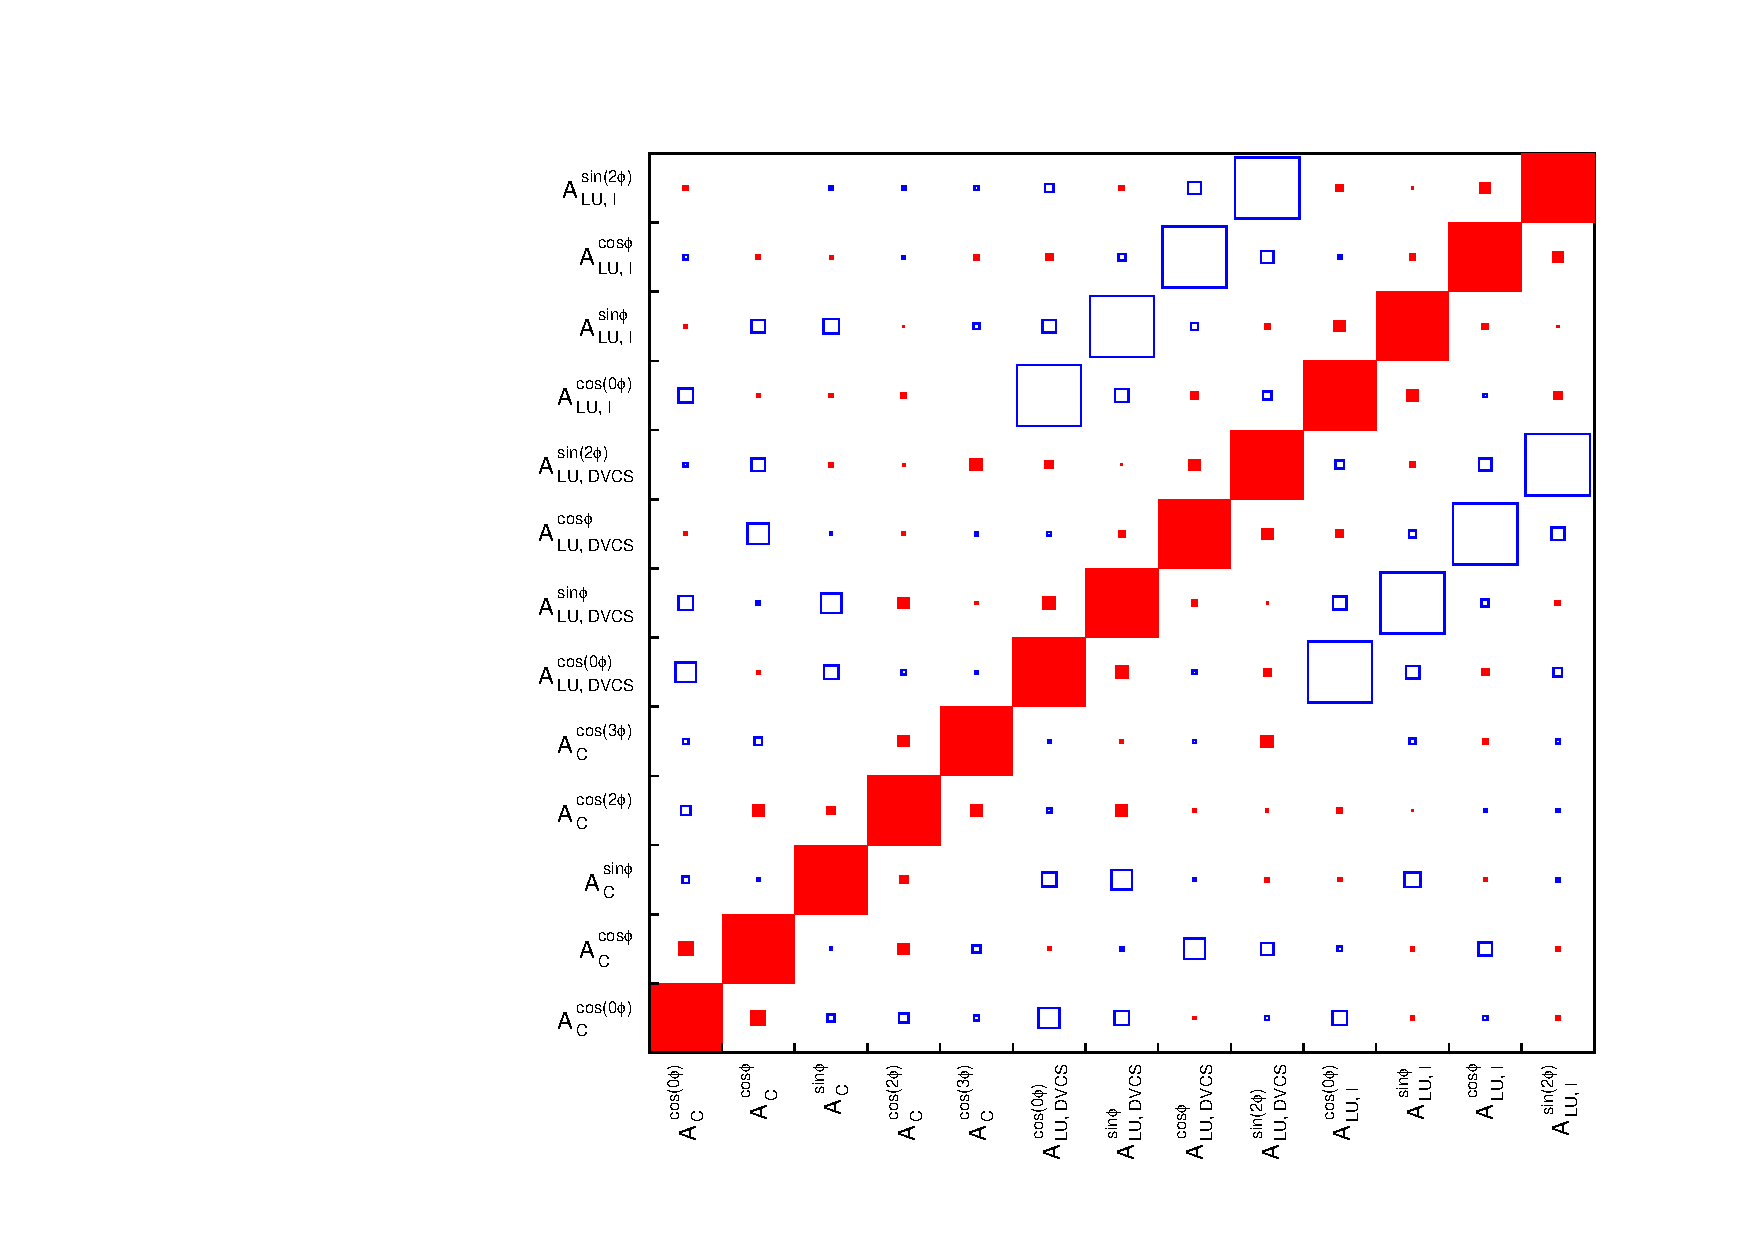
\includegraphics[width=\textwidth]{CovMat.pdf}
\caption{The covariance matrix results for the asymmetries extracted in a single bin across the whole kinematic range.}
\label{pic:covmat}
\end{figure}
